\documentclass[tikz, border=10pt]{standalone}
\usetikzlibrary{arrows.meta, patterns}

\begin{document}
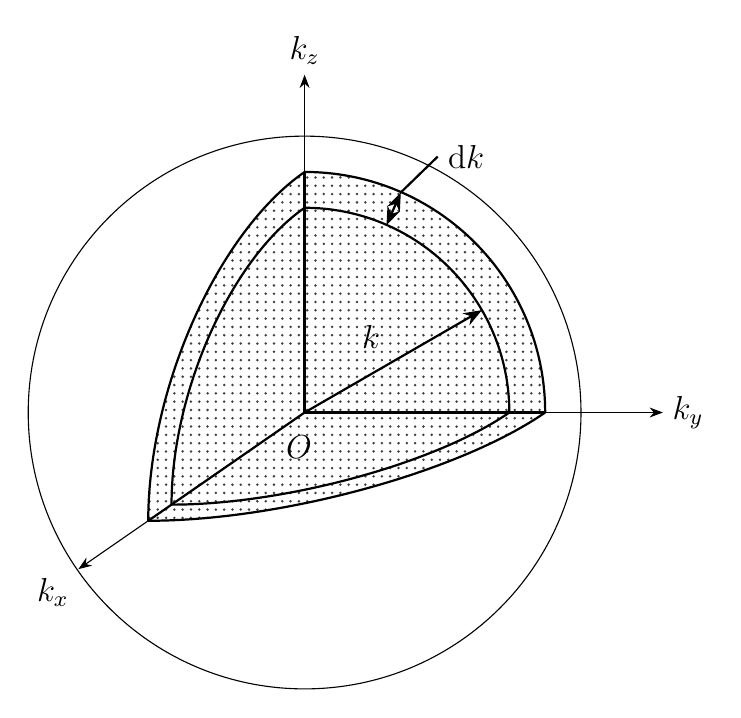
\begin{tikzpicture}[scale=1.3, >=Stealth]

  % 参数定义
  \def\Rone{2.0}   % 内球半径 k
  \def\Rtwo{2.35}  % 外球壳半径 k + dk
  \def\Rout{2.7}   % 整体球界外圈半径

  % x 轴 2D 投影向量 (左下方)
  \def\xx{-0.65}
  \def\xy{-0.45}

  % 1. 最外层球体轮廓圆
  \draw[thin] (0,0) circle (\Rout);

  % 2. 格点填充 (三个平面的截面及球壳)

  % --- (1) xOz 平面截面 (左侧竖直剖面) ---
  \begin{scope}[x={(\xx cm, \xy cm)}, y={(0cm, 1cm)}]
    % 内球 xOz 截面
    \fill[pattern=dots, pattern color=black!75]
      (0,0) -- (0,\Rone) arc (90:0:\Rone) -- cycle;
    % 球壳 xOz 截面
    \fill[pattern=dots, pattern color=black!75]
      (0,\Rone) -- (0,\Rtwo) arc (90:0:\Rtwo) -- (\Rtwo,0) -- (\Rone,0) arc (0:90:\Rone) -- cycle;
  \end{scope}

  % --- (2) xOy 平面截面 (底部水平剖面) ---
  \begin{scope}[x={(\xx cm, \xy cm)}, y={(1cm, 0cm)}]
    % 内球 xOy 截面
    \fill[pattern=dots, pattern color=black!75]
      (0,0) -- (\Rone,0) arc (0:90:\Rone) -- cycle;
    % 球壳 xOy 截面
    \fill[pattern=dots, pattern color=black!75]
      (\Rone,0) -- (\Rtwo,0) arc (0:90:\Rtwo) -- (0,\Rtwo) -- (0,\Rone) arc (90:0:\Rone) -- cycle;
  \end{scope}

  % --- (3) yOz 平面及露出的第一象限球面 ---
  % 内球 yOz 扇形/球面
  \fill[pattern=dots, pattern color=black!75]
    (0,0) -- (\Rone,0) arc (0:90:\Rone) -- (0,\Rone) -- cycle;
  % 球壳 yOz 扇形带
  \fill[pattern=dots, pattern color=black!75]
    (\Rone,0) arc (0:90:\Rone) -- (0,\Rtwo) arc (90:0:\Rtwo) -- (\Rtwo,0) -- cycle;

  % 3. 绘制轮廓实线

  % yOz 平面弧线
  \draw[thick] (0, \Rone) arc (90:0:\Rone);
  \draw[thick] (0, \Rtwo) arc (90:0:\Rtwo);

  % xOz 平面弧线 (投影)
  \begin{scope}[x={(\xx cm, \xy cm)}, y={(0cm, 1cm)}]
    \draw[thick] (0, \Rone) arc (90:0:\Rone);
    \draw[thick] (0, \Rtwo) arc (90:0:\Rtwo);
  \end{scope}

  % xOy 平面弧线 (投影)
  \begin{scope}[x={(\xx cm, \xy cm)}, y={(1cm, 0cm)}]
    \draw[thick] (\Rone, 0) arc (0:90:\Rone);
    \draw[thick] (\Rtwo, 0) arc (0:90:\Rtwo);
  \end{scope}

  % 内部剖切轴线
  \draw[thick] (0,0) -- (0, \Rtwo);
  \draw[thick] (0,0) -- (\Rtwo, 0);
  \draw[thick] (0,0) -- ({\xx*\Rtwo}, {\xy*\Rtwo});

  % 4. 坐标轴延伸线与箭头
  \draw[->, >=Stealth] (0, \Rtwo) -- (0, 3.3) node[above] {\large $k_z$};
  \draw[->, >=Stealth] (\Rtwo, 0) -- (3.5, 0) node[right] {\large $k_y$};
  \draw[->, >=Stealth] ({\xx*\Rtwo}, {\xy*\Rtwo}) -- ({\xx*3.4}, {\xy*3.4}) node[below left] {\large $k_x$};

  % 原点 O (下移避开 k_x 轴线)
  \node[below=5pt, xshift=-2pt] at (0,0) {\large $O$};

  % 5. 标注矢量 k 与厚度 dk
  \draw[->, >=Stealth, thick] (0,0) -- (1.732, 1.0) node[midway, above left=1pt] {\large $k$};
  \draw[<->, >=Stealth, thick] (0.8, 1.83) -- (0.94, 2.15);
  \draw[thick] (0.94, 2.15) -- (1.3, 2.5) node[right] {\large $\mathrm{d}k$};

\end{tikzpicture}
\end{document}